\section{Probability}
In this first lecture, we will review the basic concept of \emph{probability}. You probably have a good idea already of what probability is, however the mathematical developed in 1933 by Kolmogorov treats probability as something which satisfies three axioms, and therefore no specific definition is given. The Kolmogorov axioms are, 
\begin{itemize}
    \item $P(X_i)\geq0$ for all $i$
    \item $P(X_i~\mathrm{or}~X_j)= P(X_i) + P(X_j)$ 
    \item $\sum_{\Omega}P(X_i) =1$,
\end{itemize}
where $\Omega$ is the set of all possible, exclusive events $X_i$ and $P(X_i)$ is the probability for $X_i$ to occur. 

We can see that probability should (probably) be at least a real number between 0 and 1, but otherwise we're free to choose the interpretation. For any meaningful statistics, we need a more practical definition and like all great constructs of society (democratic elections, quantum mechanics interpretations and ``who shot first'' in ``Star wars IV: A new hope''), there are only two credible choices. 

\subsection{Frequentist probability}

The concept of probability in the \emph{frequensist} (or classical) paradigm is the one that you are most likely familiar with. As the name suggests, this definition of probability is related to the frequency with which an event occurs in repeated trials. More formally, imagine an experiment in which a series of events is observed and suppose that some ($n$) of these events can be labelled of type $X $. The probability that any single event out of a total number of $N$ events will be of type $X$ is given by the limit of the ratio, 
\begin{equation}
    P(X) = \mathrm{lim}_{N\rightarrow \infty}\frac{n}{N}.
\end{equation}
Note that we inherit some limitations with this interpretation. This concept of probability can only be applied to repeated experiments, meaning the probability only makes sense when describing an ensemble of experiments. Furthermore, the conditions of these experiments must be essentially identical. As physicists, this shouldn't be an issue for you as good science requires reproducible results. On the other hand, this definition is very objective in the sense that if everyone agrees on the definition of $X$, no-one can object to the probability for an event to be labelled $X$ - i.e the probability is independent of who is determining it.  

\subsection{Bayesian probability}

The other commonly used definition of probability is \emph{Bayesian probability}. This definition abandons the concept of frequency and instead defines probability as something which can be applied to non-repeatable experiments. The concept of Bayesian probability is based on the \emph{degree of belief} in an event $X$ occurring. Often, this is described in terms of the odds of winning a bet based on the outcome. Say for example that the odds on $X$ occurring are 4:1, meaning if you place a bet of £1 that $X$ occurs, you could either make a £4 profit or a £1 loss. If you are \emph{willing to take those odds}, as a Bayesian, then you would ascribe a probability $P(X)=1/(4+1)$ -- the ratio between the amount you would bet to the total amount you stand to win (including the original bet) under those odds.  Intuitively this makes sense, since $P(X)$ being very small means that you are almost certain $X$ will not occur and therefore require very high odds before its worth betting any money. Instead $P(X)=0.5$ means that you have have no strong belief about the outcome of $X$ and therefore willing to accept odds of 1:1. 

Note however that this definition of probability is a property of the observer and the system at the same time. It is also not a constant with time. As the observer gains more knowledge (perhaps by playing the game and placing a bet a few times), their value of $P(X)$ will change. This definition of probability is therefore \emph{subjective}. This is not necessarily a bad thing of course. Why shouldn't we update our believe about something after we gain knowledge and if you know more about how and when $X$ will occur than I do, why should your probability be the same as mine? We'll see that this definition of probability has its advantages and at the end of the day, as physicists we want to use the definitions most convenient to the problem at hand. 


\subsection{Properties of probability}

Let's quickly revisit the properties of any quantity that satisfies the Kolmogorov axioms. You would have seen these at school so there's nothing new here (hopefully). Let $P(A)$ be the probability that an exclusive event $X_i$ occurs in $A$. Now consider two non-exclusive sets $A$ and $B$ of exclusive events $X_i$. Then the probability of an event occurring in either $A$, or $B$, or in both is given by, 
\begin{equation}\label{eqn:aorb}
    P(A~\mathrm{or}~B) = P(A)+P(B)-P(A~\mathrm{and}~B),
\end{equation}
where $(A~\mathrm{or}~B)$ denotes the set of events $X_i$ which belong to either set $A$ or set $B$, or both. $(A~\mathrm{and}~B)$ denotes the set of events belonging to both.  
\begin{tcolorbox}[colback=backblue]
\textbf{Example:} Let $A$  be all even rolls of a six-sided die, and $\{X_i\}_1^6$ are the outcomes of a single roll of the die -- i.e $X_1$ denotes that a 1 is rolled, $X_2$ denotes that a 2 is rolled etc. Now let $B$ be all rolls which result in an outcome greater than or equal to 4. Then, according to Eqn.~\ref{eqn:aorb},  $P(A~\mathrm{or}~B)=\frac{1}{2}+\frac{1}{2}-\frac{1}{3}=\frac{2}{3}$. This matches what we'd expect given there are 4 outcomes that would be included in either of $A$ or $B$, namely $X_2,X_4,X_5$ and $X_6$. 
\end{tcolorbox}

The other property you'll be familiar with is related to \emph{conditional probability}, $P(A|B)$ -- the probability of $A$ given $B$. This is defined through the relationship, \begin{equation}\label{eqn:condprob}
    P(A~\mathrm{and}~B) = P(A|B)P(B) = P(B|A)P(A).
\end{equation}
We say that the sets $A$ and $B$ are \emph{independent} if $P(A|B)=P(A)$. From the definition in Eqn.~\ref{eqn:condprob}, we have that if $A$ and $B$ are independent, then, 
\begin{equation}\label{eqn:paorb}
    P(A~\mathrm{and}~B) = P(A)P(B).
\end{equation}

\subsection{Bayes theorem}
This definition brings us on to \emph{Bayes theorem} for discrete events, which states that for sets $A$ and $B$, 
\begin{equation}\label{eqn:bayesdiscrete}
     P(A|B) = \frac{P(B|A)P(A)}{P(B)},
\end{equation}
which follows from Eqn.~\ref{eqn:paorb}.
This theorem has important consequences for making decisions based on the probabilities of outcomes and can easily be forgotten when discussing them. For example, a simple pessimistic statement like ``it always rains when I bring my umbrella'', is easily checked with Bayes theorem. Let $B$ be true whenever you take your umbrella with you and $A$ be true when it's raining. Then the probability that it rains given you've brought your umbrella is the same as the probability you've brought your umbrella given that its raining multiplied by the ratio of probabilities that its raining to that of you bringing your umbrella. If it always rains where you live, then $P(A|B)=1$ since $P(A)=1$ and $A$ and $B$ are independent. However, if the probability for rain is very low, you better make sure you very rarely take your umbrella out to make such bold claim. Perhaps the most obvious but important consequence here is that the probability that it rains given you've taken your umbrella out is almost certainly not the same as the probability that you take your umbrella out given its raining -- at least if you prefer to avoid getting wet!

There is another distinction which Bayesians make use of Bayes theorem and that is concerning statements about \emph{hypotheses}. Hypothesis testing is a huge part of experimental physics (and all sciences), which we will cover in later lectures. For now, however its useful to bring up a distinction between random variables and hypotheses. To a Bayesian, $P(\theta_{i})$ represents the degree of belief in the hypothesis $H(\theta=\theta_i)$, while for frequentists, $\theta_i$ is not a random variable and therefore a probability cannot be assigned to it. To a Bayesian, the Bayes theorem can be directly applied to an experiment in which we have made a set of observations $\mathbf{X}=X_0,X_1,...$ to assign probabilities to a given hypothesis $\theta_i$, 
\begin{equation}\label{eqn:bayesexp}
    P(\theta_i|\mathbf{X}) =  P(\mathbf{X}|\theta_i)\frac{P(\theta_i)}{P(\mathbf{X})}.
\end{equation}
$P(\theta_i|\mathbf{X})$ is called the \emph{posterior probability} for hypothesis $\theta_i$, given that we have observed $\mathbf{X}$ and $P(\mathbf{X}|\theta_i)$ is the probability to observe $\mathbf{X}$, if $\theta_i$ is true. These two are related by $P(\mathbf{X})$ which is the total probability to observe $\mathbf{X}$ for any hypothesis $\theta_i$, which may or may not be known. Usually this can however be considered as a normalisation constant since summing over the LHS of Eqn.~\ref{eqn:bayesexp} for all $i$ should yield 1 if all of the $\theta_i$ form a complete and  exclusive set. Mathematically, if the hypotheses are exclusive and exhaustive (i.e they cover all possibilities), then we can calculate, 
\begin{equation}\label{eqn:norm}
    P(\mathbf{X}) = \sum_{i} P(\mathbf{X}|\theta_i)P(\theta_i)
\end{equation}
Finally the quantity $P(\theta_i)$ is called the \emph{prior probability} and represents the degree of belief in the different hypothesis \emph{before} the experiment was conducted. Clearly this will depend on the individual and studying the effect changing priors is an important part of modern Bayesian statistics. 

\begin{tcolorbox}[colback = backblue]
\textbf{Example:} The Monty Hall game show problem is a good example of using Bayes theorem to overcome our intuition. In case you don't know the problem, it goes like this. You are the contestant of a game show, presented with 3 boxes, labelled $A$, $B$ and $C$ and asked to choose one. You are told that one of the boxes contains a all-inclusive paid for trip to CERN (its an STFC funded game show) while the other two are empty. You pick box $A$ but before opening it, the game show host opens one of the remaining two boxes that she \emph{knows} doesn't contain the prize, revealing it to be empty. Given the choice of swapping your box $A$ for the remaining box, do you stick with your original choice or switch? The answer may seem like the odds are 50:50 so it doesn't matter, but let's check. 
\\
Let $P(A)$, $P(B)$ and $P(C)$ represent the  prior probabilities that the prize is inside box $A$, $B$ and $C$, respectively. Sensible prior probabilities could be $P(A)=P(B)=P(C)=\frac{1}{3}$. We want to know the posterior probabilities, given that the host opens one of the other two boxes and its empty. 
Let $H_B$ represent the case where the host opens box $B$ and $H_{C}$ the case where she opens box $C$. The probability that your box $A$ contains the prize, given that the host opens box $B$ is given by, 
\begin{equation}
    P(A|H_{B}) = \frac{P(H_{B}|A)P(A)}{P(H_{B})}
\end{equation}
The probability that the host opens $B$, given that you chose $A$ is the same as the probability that the host opens box $C$ in that case. The host knows neither box $B$ or $C$ contains the prize if the prize is in box $A$ so can choose randomly. Therefore $P(H_{B}|A)=\frac{1}{2}$. 
\\
What about $P(H_B)$? From Eqn.~\ref{eqn:norm}, this must be the sum over the conditional probabilities $P(H_{B})=P(H_B|A)P(A)+P(H_B|B)P(B)+P(H_B|C)P(C)$. The host will never pick the box that has the prize so $P(H_B|B)=0$ and the host is forced to pick $B$ if the prize is in $C$, given you've already picked $A$ so $P(H_B|C)$=1.  
This means that $P(H_B)=\frac{1}{2}\cdot\frac{1}{3}+0\cdot\frac{1}{3}+1\cdot\frac{1}{3}=\frac{1}{2}$, and therefore
\begin{equation}
    P(A|H_{B})=\frac{1/2 \cdot 1/3}{1/2}.
\end{equation}
Instead, what about the other two cases where the prize is in one of the boxes you didn't pick? Again, using Bayes theorem,
\begin{equation}
    P(C|H_B)= \frac{P(H_B|C)P(C)}{P(H_B)} = \frac{1\cdot1/3}{1/2} = \frac{2}{3}
\end{equation}
So we can see that if you pick $A$ and the host opens box $B$, the probability that the prize is in box $C$ is higher than the probability that its in box $A$, so you should switch!.  
The exact same arguments holds if instead the host opens box $C$ and of course cycling around $A, B$ and $C$ doesn't change the problem so its \emph{always} better to switch in this game show!
\end{tcolorbox}

In the above example, we calculated a collection of $P(\theta_i|\mathbf{X})$ for all $i$, where $i=A, B, C$ and $\mathbf{X}=H_{B}$. We were calculating the posterior probability \emph{distribution}. We also knew from the start that $P(\theta_i)=\frac{1}{3}$ for all $i$, which was  our prior probability \emph{distribution}. However, it may have been that we had a firmer belief, before the game show, that the prize is in a particular box (maybe the host was hovering over one of them more than the others). In general the this distribution can have a large impact on statistical (and experimental) results when using Bayesian statistics. 

We've already gotten a bit ahead of ourselves since we've talked about hypotheses and distributions of a random variable/hypotheses are without first defining what a probability distribution is. We'll cover this in the next section. 

\section{Probability distributions}

Random variables (as opposed to weather scenarios and umbrellas) are common place in HEP. Fundamental particle interactions are by their very nature probabilistic. We should therefore expect that whether we are studying cosmic rays, nuclear decays or particle collisions, we will regularly encounter random variables (energies, momenta, number of events). Note that a random variable $X$ does not need to be a single value, but may instead be multiple quantities -- in HEP, we tend to refer to this collection of quantities as an ``event''. For a sequence of events $X_1, X_2, X_3...$, we will often use vector notation $\mathbf{X}$. Note however that $\mathbf{X}$ can also refer to a repeated set of experiments and each experiment will have a single observation (e.g the total number of recorded nuclear decays in a given time window). Hopefully, it will be clear in the context as to which we mean, but the mathematics will be the same. 

The corresponding probabilities ${P(X)}_{\Omega}$ over all possible values of $X\in\Omega$ form a \emph{probability distribution}. As an example, if $X$ is the outcome of a single die roll, then $\Omega=\{X=1,X=2,X=3,X=4,X=5\}$ and $P(X)=\frac{1}{6}$ for every possible value of $X$, meaning the probability distribution is uniform. Note that of course we must have that,
\begin{equation}
    \sum_{\Omega}P(X)=1 
\end{equation}
A single event (roll) can be then thought of a random draw from such a probability distribution, and successive rolls of the die will yield a distribution of values whose frequency converges to a uniform distribution ($U)$. We will write this as $X\sim U(1,6)$.

More often than not (and essentially always) in HEP, we deal with events which are independent from one another (like the roll of an unbiased die). This means that the probability distribution of a random variable has no dependence on any other observation. 
There are a number of distributions which are common in HEP, but the one we'll talk about first will be  one you'll see over and over in your PhD -- The \emph{Poisson distribution}. 

\subsection{The Poisson distribution }

Ok, before we get onto the Poisson distribution, we first need to discuss a more fundamental distribution -- the binomial distribution. The binomial distribution describes the distribution of the number of successes ($k$) in a sequence of $n$ independent trials, where the probability of success in any trial is $p$. More generally, any sequence of experiments, each of which results in a yes/no, 1/0 or other binary result with probabilities $p$ and $q=(1-p)$ assigned to each outcome will be described by the binomial distribution, 
\begin{equation}\label{eqn:binomial}
    f(k;n,p) = \binom{n}{k} p^{k}q^{n-k},
\end{equation}
where $k$ (the number of ``yes'', ``1'' etc...) $=0,1,2...n$ and  $\binom{n}{k}=\frac{n!}{k!(n-k)!}$.
Note that I've introduced $f$ here instead of $P$ for the probability, and separated the random variable $k$ from the parameters $n,p$ with a semicolon $;$.  You may sometimes see a $|$ in place of the $;$, but in these lectures, I will only use this to mean ``\emph{given that}'' -- i.e for conditional probabilities (or related quantities). We'll use $f$ whenever discussing a probability distribution (which will be more important to distinguish later when we get to \emph{probability densities}. 

In HEP, we often deal with counting events of a certain type. For example, the LUX experiment aimed to detect the presence of dark matter by counting the the number of events in which a dark matter particle interacted with a Xenon nucleus from a vast amount of liquid Xenon, which is shielded from other radiation sources. The number of dark matter particles passing through the earth at any given moment is expected to be relatively large, however the probability that one of these particles interacts is extremely small. In this circumstance, we can use a limit case of the binomial distribution where $n\rightarrow \infty$, and $p\rightarrow 0$ such that the product $\lambda = np$ is constant. 

Let's re-write Eqn.~\ref{eqn:binomial} substituting $p=\frac{\lambda}{n}$, 
\begin{eqnarray}
    f(k;n,p) & = & \frac{n!}{k!(n-k)!}\left(\frac{\lambda}{n}\right)^{k}\left(1-\frac{\lambda}{n}\right)^{n-k}\\
    & = & \frac{\lambda^{k}}{k!}\frac{n!}{(n-k)!}\left(\frac{1}{n}\right)^{k}\left(1-\frac{\lambda}{n}\right)^{n-k}
\end{eqnarray}
Now lets look at the middle terms in the product,
\begin{eqnarray}
    \frac{n!}{(n-k)!}\left(\frac{1}{n}\right)^{k} & = & 
    \frac{n(n-1)(n-2)...(n-k+1)(n-k)(n-k-1)...(2)}
    {n^k(n-k)(n-k-1)...(2)}\\
    & = & \frac{n}{n^{k}}(n-1)(n-2)...(n-k+1)\\
    & = & \bcancel{\frac{n^{k}}{n^{k}}}\left(1-\frac{1}{n}\right)\left(1-\frac{2}{n}\right)...\left(1-\frac{k+1}{n}\right) = A
\end{eqnarray}
Now lets look at the last term, 
\begin{eqnarray}
\left(1-\frac{\lambda}{n}\right)^{n-k} & = & \left(1-\frac{\lambda}{n}\right)^{n}\left(1-\frac{\lambda}{n}\right)^{-k} = B
\end{eqnarray}
Now lets look at what happens when $n\rightarrow \infty$. The second term in $B$ will tend to 1 since $\lambda$ is constant. The first term, is the usual expression for the exponential function, 
\begin{equation}
    e^{x} = \mathrm{lim}_{n\rightarrow\infty}\left(1+\frac{x}{n}\right)^n,
\end{equation}
so $B\rightarrow e^{-\lambda}$ as $n\rightarrow \infty$.
It should be easy to see also that $A\rightarrow 1$ as $n\rightarrow \infty$, so that finally, 
\begin{equation}
    f(k;n,p)  \rightarrow f(k;\lambda) = \frac{\lambda^{k}}{k!}e^{-\lambda}
\end{equation}
as $n\rightarrow \infty$, which is the Poisson distribution. We can take a look at this distribution using some simple code to generate it. Below is a snippet of code using the \textsf{numpy.random.poisson} function, which generates a vector of random integers (``toys'') according to the Poisson distribution, for a given value of $\lambda$. By generating a large number of them we can determine the frequency (i.e the probability) to get a given integer, and plot what that frequency is for each integer. 
\begin{lstlisting}[style = Python]
import numpy
import matplotlib.pyplot as plt
plt.rcParams.update({'font.size': 14})

# 5 different values of \lambda
lambdas = numpy.arange(0.1,10,2.0)
colors  = ["red","crimson","purple",
          "mediumslateblue","blue"]

# generate the distributions with MC
for lamb,col in zip(lambdas,colors):
 poisson_distribution = numpy.random.poisson(lamb,size=10000)
 plt.hist(poisson_distribution,bins=20,range=(0,20),\
    density=True,color=col,linewidth=2.\
    ,histtype='step',label="$\lambda=$%.1f"%lamb)

plt.xlabel("$k$")
plt.ylabel("$f(k,\lambda$)")
plt.legend()
plt.show()
\end{lstlisting}

The distributions are shown in Fig.~\ref{fig:poissondistributions}. You can see that as $\lambda$ increases, the distribution looks more symmetric around its mode and that this mode gets closer to the value of $\lambda$. This is an important feature of the Poisson distribution that we'll come to later on in the lectures. In the Poisson distribution, our random variable $X=k$ and we write that $k$ is distributed as a Poisson distribution with parameter lambda $k\sim \mathrm{Poisson}(\lambda)$ (just to avoid writing $f(k;\lambda)$ all the time). 

\begin{figure}[hbt!]
    \centering
    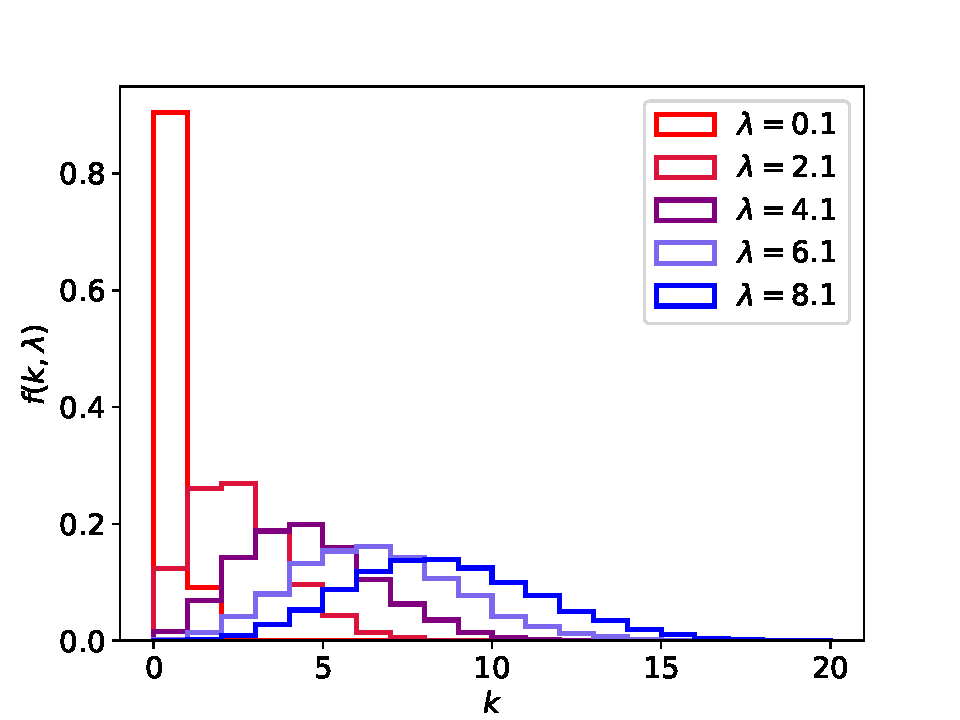
\includegraphics[width=0.8\textwidth]{figures/Probability/PoissonProbs.pdf}
    \caption{Poisson probability distribution $f(k;\lambda)$ for different values of the parameter $\lambda$. The distributions are produced by randomly generating 10,000 values (toys) of $k$ according to a Poisson distribution with parameter $k$, and creating the histogram of the results.}
    \label{fig:poissondistributions}
\end{figure}

\subsection{Continuous random variables and probability densities}

We can generalize probabilities (and distributions of probability) for events to probability distributions of \emph{continuous} random variables. A continuous random variable  is one whose possible values cover continuous intervals, for example $X\in\mathbb{R}$. In this case, we need to define something called a \emph{probability density function}. 

Suppose we measure the energy $E$ of cosmic ray particles. Due to the underlying quantum mechanics of interactions with the atmosphere, there will be a probability that the particle has a particular energy within some finite range $P(E \in (E+\delta E)$. As the energy is a continuous variable, we are free to choose $\delta E$ as small as we like. If there is a continuous function for all values of $E>0$ which represents the limit as $\delta E\rightarrow 0$, 
\begin{equation}
    f(E) = \mathrm{lim}_{\delta E\rightarrow 0}\frac{P(E \in (E+\delta E)}{\delta E}
\end{equation}
we call that function the \emph{probability density function} or p.d.f. The p.d.f must be normalised analogously to the discrete case such that, \begin{equation}
    \int_{\Omega} f(E)dE = 1, ~\mathrm{where} ~E\in\Omega.
\end{equation} 
Of course, as with the discrete case, we can measure multiple continuous quantities $\mathbf{X}$ in which case $d\mathbf{X}=dXdYdZ,...$ represents an infinitesimal volume. 

We can define two more distributions related to the probability density. The first is the \emph{cumulative distribution}, defined by the integral, 
\begin{equation}
    F(X) = \int_{X_{a}}^X f(X')dX' 
\end{equation}
where $X_a \leq X \leq X_b$, and $f(X)$ is the probability density distribution of $X$. Clearly then $F(X_a)=0$ and $F(X_b)=1$. We can interpret $F(X_{1})$ as the probability that $X\leq X_1$.  The cumulative distribution will be used later when we discuss $p$-values.

If the probability density function has more than one random variable, we can define a projection onto a fewer number of variables, which is called the \emph{marginal density}. For example, if we have a probability density $f(X,Y)$, the projection onto the $X$ variable is given by, 
\begin{equation}\label{eqn:marginal}
    g(X) = \int_{Y_{a}}^{Y_{b}} f(X,Y)dY 
\end{equation}
where $Y_a \leq Y \leq Y_b$.

We can also use Bayes theorem for continuous random variables. If $f(X,Y)$ is the probability density for two variable $X$ and $Y$, with marginal densities $g(X)$ and $h(Y)$, then Eqn.~\ref{eqn:bayesdiscrete} becomes, 
\begin{equation}
    q(Y|X) = \frac{p(X|Y)h(Y)}{g(X)},
\end{equation}
where $q(Y|X)$ and $p(X|Y)$ are the conditional probabilities defined through the relationship 
\begin{equation}
   f(X,Y)= p(X|Y)h(Y) = q(Y|X)g(X).
\end{equation}

\subsection{Moments of probability distributions}

Probability density distributions can be used to obtain useful information about a particular random variable, or functions of random variables. For example, the mean value of a random variable $X$ (or its \emph{expectation value} under $f(X)$ is given by, 
\begin{equation}\label{eqn:expectation}
    E[X] = \int_{\Omega} Xf(X)dX,
\end{equation}
where $E[\cdot]$ is the expectation operator. 
Similarly, any function of $X$, $g(X)$ has an expectation value $E[g]$ under $f(X)$ of,
\begin{equation}
    E[g] = \int_{\Omega} g(X)f(X)dX
\end{equation}
It should be obvious that the expectation is a \emph{linear} operator, since, 
\begin{equation}\label{eqn:linearexpectation}
    E[a\cdot g(X)+b\cdot h(Y)] = a\cdot E[g(X)]+b\cdot E[h(Y)]
\end{equation}
If the two variables $X$ and $Y$ are \emph{independent} then we also have that $ E[X\cdot Y] = E[X] E[Y]$.

The expectation value (mean) is often referred to as the \emph{first moment} of the distribution of $X$, but of course we can define higher moments too. For example, the expectation of the function $g(X)=(X-E[X])^{2}$ is called the \emph{variance} of $X$ under $f(X)$, 
\begin{equation}\label{eqn:variance}
    V(X) = E[(X-E[X])^{2}] = \int_{\Omega} (X-E[X])^2f(X)dX
\end{equation}
You will also have come across the term \emph{standard deviation}, $\sigma = \sqrt{V(X)}$. Note that the variance (or the standard deviation) is \emph{not} a linear operator. However, we do have the following properties, 
\begin{equation}
 V(X+a) = V(X) ~\mathrm{and}~ V(aX)=a^{2}V(X),
\end{equation}
when $a$ is a constant value. 

There are equivalents of the expectation and variance for discrete random variables too, $E[X]=\bar{X}=\sum_{\Omega}Xf(X)$, and $V(X)=\sum_\Omega (X-E[X])^2f(X)$.
\begin{tcolorbox}[colback = backblue]
\textbf{Example:} The expectation and variance of a discrete random variable $k$ distributed as a Poisson distribution can be calculated using the discrete versions of the formula given in Eqns.~\ref{eqn:expectation} and~\ref{eqn:variance}.
\begin{eqnarray}
E[k] & = & \sum_{k=0}^{\infty}ke^{-\lambda}\frac{\lambda^{k}}{k!}
      =  e^{-\lambda}\sum_{k=0}^{\infty}k\frac{\lambda^{k}}{k!}
      =  e^{-\lambda}\lambda e^{\lambda} \\
      & = & \lambda,
\end{eqnarray}
and,
\begin{eqnarray}
V(k) & = & \sum_{k=0}^{\infty}(k-\lambda)^2 e^{-\lambda}\frac{\lambda^{k}}{k!} \\
      & = & e^{-\lambda}\sum_{k=0}^{\infty}k^{2}\frac{\lambda^{k}}{k!}
      -2\lambda e^{-\lambda}\sum_{k=0}^{\infty}k\frac{\lambda^{k}}{k!}
      + \lambda^{2} e^{-\lambda}\sum_{k=0}^{\infty}\frac{\lambda^{k}}{k!} \\
      & = & \lambda+\lambda^{2} - 2\lambda^{2}+\lambda^{2} \\
      & = & \lambda
\end{eqnarray}
using the identities $(x^2+x)e^{x}=\sum_{k=0}^{\infty}k^{2}\frac{x^{k}}{k!}$, $xe^{x}=\sum_{k=0}^{\infty}k\frac{x^{k}}{k!}$, and $e^{x}=\sum_{k=0}^{\infty}\frac{x^{k}}{k!}$. So for $k\sim\mathrm{Poisson}(\lambda)$, we have $E[k]=V(k)=\lambda$.  
\end{tcolorbox}

Of course, there are other moments we can calculate which describe more properties of the probability distribution we're interested in. Specifically, 
\begin{equation}
    \mu_{n} = E[X^{n}] ~ \mathrm{is~the}~n^{\mathrm{th}}~\mathrm{algebraic~moment},
\end{equation}
and,
\begin{equation}
    \nu_{n} = E[(X-E[X])^{n}] ~ \mathrm{is~the}~n^{\mathrm{th}}~\mathrm{central~ moment}.
\end{equation}
Then we have that $E[X]=\mu_{1}$ and $V(X)=\nu_{2}$.
Often you'll see quantities which are constructed from these moments. For example, the \emph{skewness} of a probability distribution is given by, 
\begin{equation}
    \gamma = \frac{\nu_{3}}{(\nu_2)^{3/2}},
\end{equation}
which describes an asymmetry in the distribution. 
We can also determine moments of multidimensional distributions too. For example for a probability distribution $f(X,Y)$, the algebraic moment of order $m$ in $X$ and $n$ in $Y$ is $\mu_{mn}=E[X^{m}Y^{n}]$. The most common moment you'll come across is the \emph{co-variance}, which for an $M$ dimensional probability distribution $f(\mathbf{X})$, is the central moment of order 1 in two variables $X_{i}, X_{j}$ and order 0 for the remaining $M-2$ variables, 
\begin{equation}
    \mathrm{covariance}(X_{i},X_{j}) = \nu^{ij}_{1,1} = E[(X_{i}-E[X_{i}])(X_{j}-E[X_{j}])], 
\end{equation}
and the \emph{correlation coefficient} is given by 
\begin{equation}
    \mathrm{correlation}(X_{i},X_{j}) = \rho(X_{i},X_{j}) = \frac{\nu^{ij}_{1,1}}{\sqrt{v^{i}_{2}v^{j}_{2}}} , 
\end{equation}
where $v^{i}_{2}$, and $v^{j}_{2}$ are the variance of $X_{i}$ and $X_{j}$ respectively. The correlation coefficient will be $-1\leq \rho \leq 1$. 
Two variables $X$, $Y$ which are independent under $f(X,Y)$ will have a correlation coefficient of 0. The reverse is however not necessarily true so you should remember that \emph{independence} is a stronger statement than \emph{uncorrelated} (see problems for an example).  

\subsection{Compositions of probability distributions}

Compositions of random variables can be used to determine the distributions of derived quantities in HEP. We haven't covered what we mean by a ``measurement'' yet but you'll know that any measurement of a physical quantity is meaningless without an associated  ``uncertainty''. Actually, uncertainty in the sense we need for HEP won't be covered until the last sections of these lectures. However, you are probably aware of the concept at least in relation to the variance of a random variable. Often you'll have come across the idea of uncertainty being associated to the standard deviation -- $\sigma_{X} = \sqrt{V(X)}$. Quite correctly, if $X$ is a measured quantity, more often than not, it will be a random variable and we'll see that the standard deviation of this variable can be a pretty good approximation to a more concrete definition of uncertainty. You'll also have come across the concept of propagating uncertainties for quantities built from random variables such as the sum of two random variables $X$, $Y$. We already know that $E[X+Y]=E[X]+E[Y]$ by the linearity of expectation, but for the variance, the formula you know is, 
\begin{equation}\label{eqn:quadraturesum}
    V(X+Y) = V(X)+V(Y). 
\end{equation}
We'll see where this comes from. 

Suppose $X\sim f(X)$ and $Y\sim g(Y)$ are two independent random variables and $U=X+Y$. What is the probability distribution $p(U)$ of $U$?. First, we change variables to, \begin{equation}
    U = X+Y, ~V = X. 
\end{equation}
The probability distribution $h(U,V)$ is defined by, 
\begin{equation}
    h(U,V)dUdV = f(X)g(Y)dXdY,
\end{equation}
since the probability (not necessarily the density however) must be invariant under a change of variables.  for a change of variables, the infinitesimal volume $dXdY$ changes as, 
\begin{equation}
    dXdY =  \left|\mathrm{det} \begin{bmatrix} 
    \frac{\partial U}{\partial X} & \frac{\partial U}{\partial Y}\\
    \frac{\partial V}{\partial X} & \frac{\partial V}{\partial Y}
   \end{bmatrix}\right| ^{-1} dUdV=  dUdV
\end{equation}
then we have 
\begin{equation}
    h(U,V)dUdV = f(V)g(U-V)dUdV ~\implies h(U,V) = f(V)g(U-V).
\end{equation}
Recall that to obtain the marginal density $p(U)$, we integrate over $V$ (see Eqn.~\ref{eqn:marginal}) to obtain, 
\begin{equation}\label{eqn:sumsofrandoms}
    p(U) = \int_{-\infty}^{+\infty}h(U,V)dV =  \int_{-\infty}^{+\infty}f(U)g(U-V)dV.
\end{equation}
Note that we have relied on the fact that the change of variables $X,Y\rightarrow U,V$ is a \emph{bijection} (1 to 1 mapping). If it were not the case, then we could split the integral into segments over which each transformation is a bijection. 

\begin{tcolorbox}[colback=backblue]
\textbf{Example:} In the case that $X~\sim\phi(X;\mu_{X},\sigma_{X})$ and $Y~\sim\phi(Y;\mu_{Y},\sigma_{Y})$, where 
\begin{equation}\label{eqn:gaussian}
    \phi(x;\mu,\sigma) = \dfrac{1}{\sigma\sqrt{2\pi}} e^{-\dfrac{(x-\mu)^2}{2\sigma^{2}}}
\end{equation}
is the \emph{Gaussian} (or normal) distribution, we can find the probability distribution of $U=X+Y$. Plugging $\phi(\cdot)$ into Eqn.~\ref{eqn:sumsofrandoms} we find, 
\begin{eqnarray}
    p(U) & = & \int_{-\infty}^{+\infty}\frac{1}{\sigma_{X}\sqrt{2\pi}} \mathrm{exp}\left[{-\frac{(V-\mu_{X})^2}{2\sigma_{X}^{2}}}\right]\dfrac{1}{\sigma_{Y}\sqrt{2\pi}} \mathrm{exp}\left[{-\frac{(U-V-\mu_{Y})^2}{2\sigma_{Y}^{2}}}\right]dV\\
    & = & \int_{-\infty}^{+\infty} 
    \frac{1}{\sqrt{2\pi}\sqrt{2\pi}\sigma_{X}\sigma_{Y}} 
    \mathrm{exp}\left[{-\frac{(V-\mu_{X})^2}{2\sigma_{X}^{2}}-\dfrac{(U-V-\mu_{Y})^2}{2\sigma_{Y}^{2}}}\right]dV\\
    & = &   \int_{-\infty}^{+\infty} 
    \frac{1}{\sqrt{2\pi}\sqrt{2\pi}\sigma_{X}\sigma_{Y}} 
    \mathrm{exp}\left[
    -\frac{\sigma_{Y}^{2}(V-\mu_{X})^2 +\sigma_{X}^{2}(U-V-\mu_{Y})^2} {2\sigma_{X}^{2} \sigma_{Y}^{2}}
    \right]dV\\
    & = &   \int_{-\infty}^{+\infty} 
    \frac{1}{\sqrt{2\pi}\sqrt{2\pi}\sigma_{X}\sigma_{Y}} 
    \mathrm{exp}\left[
    A 
    \right]dV\\
\end{eqnarray}    
Expanding the exponent,
\begin{eqnarray}
    A
    & = & \frac{-(\sigma_{X}^{2}+\sigma_{Y}^{2})V^{2}+2\left(\sigma_{X}^{2}(U-\mu_{Y})+\sigma_{Y}^{2}\mu_{X}\right)V -\sigma_{X}^{2}(U^{2}+\mu_{Y}^{2}-2U\mu_{Y})-\sigma_{Y}^{2}\mu_{X}^{2}}{2\sigma_{X}^{2} \sigma_{Y}^{2}}\\
    & = & \frac{-\sigma_{U}^{2}V^{2}+2\left(\sigma_{X}^{2}(U-\mu_{Y})+\sigma_{Y}^{2}\mu_{X}\right)V -\sigma_{X}^{2}(U^{2}+\mu_{Y}^{2}-2U\mu_{Y})-\sigma_{Y}^{2}\mu_{X}^{2}}{{2\sigma_{X}^{2} \sigma_{Y}^{2}}}\\
    & = & \frac{-V^{2}+2\left(\sigma_{X}^{2}(U-\mu_{Y})+\sigma_{Y}^{2}\mu_{X}\right)\frac{V}{\sigma_{U}^{2}} -\dfrac{\sigma_{X}^{2}}{\sigma_{U}^{2}}(U-\mu_{Y})^{2}-\frac{\sigma_{Y}^{2}\mu_{X}^{2}}{\sigma_{U}^{2}}}{2\left(\frac{\sigma_{X} \sigma_{Y}}{\sigma_{U}}\right)^{2}},
 \end{eqnarray}   
where we have defined $\sigma_{U}^{2}=\sigma_{X}^{2}+\sigma_{Y}^{2}$. Now we can complete the square for $V$, to get, 
\begin{eqnarray}
    A & = & \frac{ 
    -\left(V-\frac{\sigma_{X}^{2}(U-\mu_{Y})+\sigma_{Y}^{2}\mu_{X}}{\sigma_{U}^{2}}\right)^{2} +\left(\frac{\sigma_{X}^{2}(U-\mu_{Y})+\sigma_{Y}^{2}\mu_{X}}{\sigma_{U}^{2}}\right)^{2} 
    - \frac{\sigma_{X}^{2}(U-\mu_{Y})^{2}+\sigma_{Y}^{2}\mu_{X}^{2}}{\sigma_{U}^{2}}}
    {2\left(\frac{\sigma_{X} \sigma_{Y}}{\sigma_{U}}\right)^{2}}.
\end{eqnarray}
If we plug $A$ back into the exponent we get, 
\begin{eqnarray}
  \mathrm{exp[A]} & = & \mathrm{exp}\left[\frac{ \left(\frac{\sigma_{X}^{2}(U-\mu_{Y})+\sigma_{Y}^{2}\mu_{X}}{\sigma_{U}^{2}}\right)^{2} 
    - \frac{\sigma_{X}^{2}(U-\mu_{Y})^{2}+\sigma_{Y}^{2}\mu_{X}^{2}}{\sigma_{U}^{2}}}
    {2\left(\frac{\sigma_{X} \sigma_{Y}}{\sigma_{U}}\right)^{2}} \right] \times \\ 
    & & 
    \mathrm{exp}\left[\frac{ 
    -\left(V-\frac{\sigma_{X}^{2}(U-\mu_{Y})+\sigma_{Y}^{2}\mu_{X}}{\sigma_{U}^{2}}\right)^{2}}{2\left(\frac{\sigma_{X} \sigma_{Y}}{\sigma_{U}}\right)^{2}}\right]
\end{eqnarray}
The first exponential is constant in $V$, so it can come outside of the integral. Furthermore, for the normalisation term, we have, 
\begin{eqnarray}
\frac{1}{\sqrt{2\pi}\sqrt{2\pi}\sigma_{X}\sigma_{Y}} & = & \frac{1}{\sqrt{2\pi}\sigma_{U}} \frac{\sigma_{U}}{\sqrt{2\pi}\sigma_{X}\sigma_{Y}}
\end{eqnarray}
so then, 
\begin{eqnarray}
p(U) & = & \frac{1}{\sqrt{2\pi}\sigma_{U}}\mathrm{exp}\left[\frac{ \left(\frac{\sigma_{X}^{2}(U-\mu_{Y})+\sigma_{Y}^{2}\mu_{X}}{\sigma_{U}^{2}}\right)^{2} 
    - \frac{\sigma_{X}^{2}(U-\mu_{Y})^{2}+\sigma_{Y}^{2}\mu_{X}^{2}}{\sigma_{U}^{2}}}
    {2\left(\frac{\sigma_{X} \sigma_{Y}}{\sigma_{U}}\right)^{2}} \right] \times \\ 
    & & 
    \int_{-\infty}^{+\infty}\dfrac{1}{\sqrt{2\pi}\frac{\sigma_{X}{\sigma_{Y}}}{\sigma_{U}}}
    \mathrm{exp}\left[\frac{ 
    -\left(V-\frac{\sigma_{X}^{2}(U-\mu_{Y})+\sigma_{Y}^{2}\mu_{X}}{\sigma_{U}^{2}}\right)^{2}}{2\left(\frac{\sigma_{X} \sigma_{Y}}{\sigma_{U}}\right)^{2}}\right]dV.
\end{eqnarray}
\end{tcolorbox}
\begin{tcolorbox}[colback=backblue]
The term inside the integral is just a Gaussian distribution in $V$ (with $\sigma=\frac{\sigma_{X}\sigma_{Y}}{\sigma_{U}}$), so the integral just yields 1. Therefore, 
\begin{eqnarray}
p(U) & = & \frac{1}{\sqrt{2\pi}\sigma_{U}}\mathrm{exp}\left[\frac{ \left(\frac{\sigma_{X}^{2}(U-\mu_{Y})+\sigma_{Y}^{2}\mu_{X}}{\sigma_{U}^{2}}\right)^{2} 
    - \frac{\sigma_{X}^{2}(U-\mu_{Y})^{2}+\sigma_{Y}^{2}\mu_{X}^{2}}{\sigma_{U}^{2}}}
    {2\left(\frac{\sigma_{X} \sigma_{Y}}{\sigma_{U}}\right)^{2}} \right]\\
    & = & 
    \frac{1}{\sqrt{2\pi}\sigma_{U}}\mathrm{exp}\left[\frac{ \left({\sigma_{X}^{2}(U-\mu_{Y})+\sigma_{Y}^{2}\mu_{X}}\right)^{2} 
    - \sigma_{U}^{2}\left({\sigma_{X}^{2}(U-\mu_{Y})^{2}+\sigma_{Y}^{2}\mu_{X}^{2}}\right)}
    {2\sigma_{U}^{2}\left({\sigma_{X} \sigma_{Y}}\right)^{2}} \right]\\
    & = & 
    \frac{1}{\sqrt{2\pi}\sigma_{U}}\mathrm{exp}\left[\frac{ \left({\sigma_{X}^{2}(U-\mu_{Y})+\sigma_{Y}^{2}\mu_{X}}\right)^{2} 
    - \sigma_{U}^{2}\left({\sigma_{X}^{2}(U-\mu_{Y})^{2}+\sigma_{Y}^{2}\mu_{X}^{2}}\right)}
    {2\sigma_{U}^{2}\left({\sigma_{X} \sigma_{Y}}\right)^{2}} \right]\\
    & = & 
    \frac{1}{\sqrt{2\pi}\sigma_{U}}\mathrm{exp}\left[-\frac{ (U-(\mu_{X}+\mu_{Y})^{2})(\sigma_{X}\sigma_{Y})^{2}}
    {2\sigma_{U}^{2}\left({\sigma_{X} \sigma_{Y}}\right)^{2}} \right]\\
     & = & 
    \frac{1}{\sqrt{2\pi}\sigma_{U}}\mathrm{exp}\left[-\frac{ (U-(\mu_{X}+\mu_{Y})^{2})}
    {2\sigma_{U}^{2}} \right],
\end{eqnarray}
which is a Gaussian distribution with $\mu_{U}=\mu_{X}+\mu_{Y}$, and $\sigma_{U}^{2}=\sigma_{X}^{2}+\sigma_{Y}^{2}$ or $V(U)=V(X)+V(Y)$.
\end{tcolorbox}

So there we have shown that the sum of two random normal variables yields another normally distributed random variable and we've verified Eqn.~\ref{eqn:quadraturesum}! We can check that our calculation is correct in an example. The following \textsf{Python3} code will generate toys from two Gaussian distributions $X\sim\phi(X;10,1)$, $Y\sim\phi(Y;-6,0.5)$ using the \textsf{numpy.random.normal} function. The generated values of $X$ and $Y$ are summed, and those values are filled into a histogram. We should be able to see that this distribution looks like another Gaussian distribution with $\mu=-6+10=4$ and $\sigma=\sqrt{0.5^2+1^2}=1.1$. 

\begin{lstlisting}[style = Python]
import numpy
import matplotlib.pyplot as plt

def gaus(x,mu,sigma):
 A = (1./(sigma*(2*numpy.math.pi)**0.5))
 B = numpy.math.exp(-(x-mu)*(x-mu)/(2*sigma*sigma))
 return A*B
 
muX, sigmaX = 10., 1.
muY, sigmaY = -6., 0.5

# generate toy values from the two Gaussian distributions and sum
toys_X = numpy.random.normal(muX,sigmaX,1000)
toys_Y = numpy.random.normal(muY,sigmaY,1000)
toys_U = toys_X+toys_Y

# plot the toys and compare to the expected Gaussian distributions
x = numpy.arange(-10,20,0.1)

plt.hist(toys_X,100,(-10,20),density=True,color='green')
plt.hist(toys_Y,100,(-10,20),density=True,color='red')
plt.hist(toys_U,100,(-10,20),density=True,color='cyan')

# according to our calculation for the sum of two Gaussian variables
mu    = muX + muY
sigma = ((sigmaX)**2 + (sigmaY)**2)**0.5

plt.plot(x,[gaus(xx,mu,sigma) for xx in x],color='black')
print("mu=%.1f, sigma=%.1f"%(mu,sigma))

plt.xlabel("$U$")
plt.ylabel("$\\phi(U)$")
plt.show()
\end{lstlisting}

The output of the code is shown in Fig.~\ref{fig:gaussiansum}. 
\begin{figure}[hbt!]
    \centering
    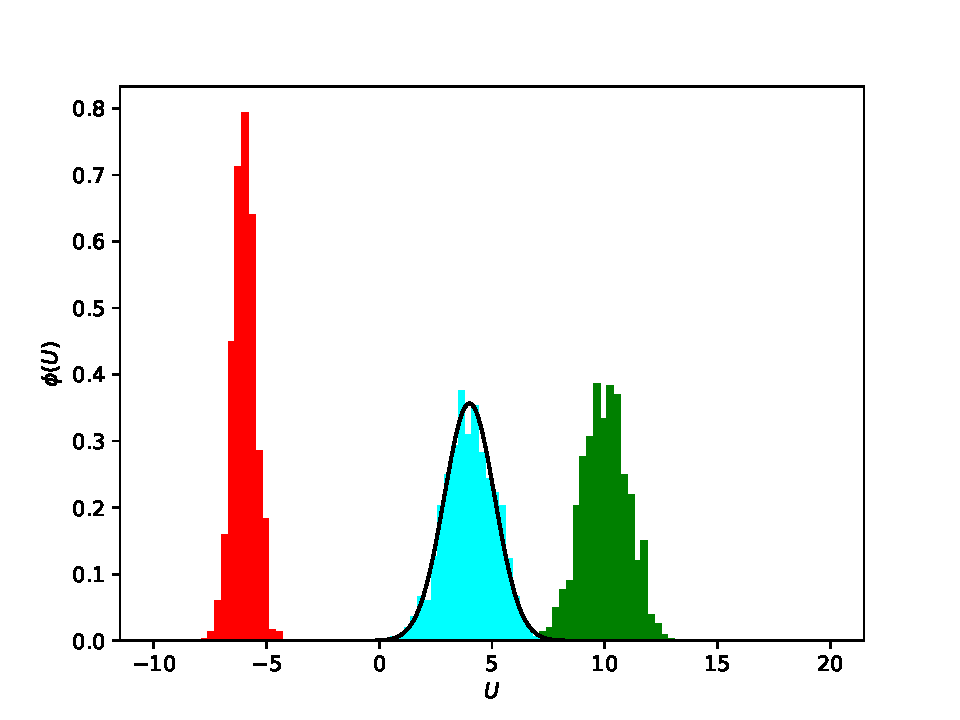
\includegraphics[width=0.8\textwidth]{figures/Probability/GaussianSum.pdf}
    \caption{Distribution of toys generated from a Gaussian with $\mu=-6,~\sigma=0.5$ (red histogram) and $\mu=-10,~\sigma=1$ (green histogram). The cyan histogram shows the distrubtion of the sum of the toys, and the black line shows the Gaussian distribution with $\mu=-6+10=4$ and $\sigma=\sqrt{0.5^2+1^2}=1.1$. }
    \label{fig:gaussiansum}
\end{figure}
Be warned however, that compositions of even Gaussian random variables doesn't always result in something Gaussian. For example, if $X\sim \phi(X;0,1)$ and $Y\sim \phi(Y;0,1)$ and $U=\frac{X}{Y}$, then (as you'll show in one of the problems) $p(U)$ is a Cauchy distribution, 
\begin{equation}
    p(U) = \dfrac{1}{\pi(1+U^{2})},
\end{equation}
which has no mean value and infinite variance!. In this case, the usual error propagation formula can be quite misleading. 
 

\section{The convergence law of large numbers}

You are certainly aware of the concept of \emph{convergence}. We used it already to demonstrate how the Poisson distribution arises from the binomial distribution when the probability of success is very small. In statistics, there are different kinds of convergence so we need to be careful to specify the sense in which something converges to another. The two most common senses in statistics are \emph{convergence in distribution} and \emph{convergence in probability}. First, we will define these two senses, without much discussion as to their application. This is because in the end, as particle physicists, the main result we care about is the \emph{central limit theorem}, which turns out to be extremely powerful for testing hypotheses and measuring physical properties -- i.e for the main job of a particle physicist. 
\paragraph{Convergence in distribution:}
Consider a sequence of random variables $\{X_{1},X_{2},...,X_{n}\}$ with cumulative distribution functions $\{F(X_{1}),F(X_2),...,F(X_{n})\}$. The sequence $X_{n}$ converges in distribution as $n\rightarrow \infty$ to $X$, with cumulative distribution $F$ if for every point where $F(X)$ is continuous, 
\begin{equation}
    \mathrm{lim}_{n\rightarrow \infty}F_{n}(X) = F(X).
\end{equation}
\paragraph{Convergence in probability:}
We say that the sequence of random variables $\{X_{1},X_{2},...,X_{n}\}$, \emph{converges in probability} to $X$ if for any $\epsilon > 0$ and $\delta>0$, there exists a value of $N$ such that, 
\begin{equation}
    P(|X_{n}-X|>\epsilon) < \delta, 
\end{equation}
for all $n\geq N$. This definition of convergence is stronger than convergence in distribution since nothing about the distance between $X$ and $X_{n}$ is implied in the other definition. Convergence in probability implies convergence in distribution. 

The most important application of convergence is in the law of large numbers, which concerns the convergence of the sample mean. Let $\{X_{1},...X_{N}\}$ be a sequence of \emph{independent} random variables, each having the same mean $\mu_{1}$ and variances $\nu^{i}_{2}$. We determine the \emph{sample mean}, $\bar{X}$ as, 
\begin{equation}
    \bar{X} = \frac{1}{N}\sum_{i=1}^{N}X_{i}.
\end{equation}
Note that this is not the same as $\mu_{1}$ since this refers to the expectation value of $X_i$ under their probability distributions. If $\mu_{1}$ exists, then if either, 
\begin{eqnarray}
  \mathrm{lim}_{N\rightarrow \infty} \left[\frac{1}{N^{2}}\sum_{i=1}^{N}\nu^{i}_{2} \right] = 0 & \mathrm{\textbf{or}} & \mathrm{lim}_{N\rightarrow \infty}\left[\sum_{i=1}^{N}\frac{\nu^{i}_{2}}{i^{2}} \right] \mathrm{~is~finite}, 
\end{eqnarray}
then $\bar{X}$ converges in probability to $\mu_{1}$. 

\subsection{The central limit theorem}
So far we have talked separately convergence of sequences of  distributions and the convergence of the sample mean of independent random variables. The \emph{central limit theorem} (CLT) states how the sum of independent random variables (for example as in sample means) is \emph{distributed} in the limit of large $N$. 
Suppose we have a sequence of independent random variables $X_{i}$, each from a distribution with mean $\mu_{1}^{i}$ and variance $\nu_{2}^{i}$. Now let, 
\begin{equation}\label{eqn:clt}
   T_{N}= \dfrac{\bar{X}N - \sum_{i=1}^{N} \mu_{1}^{i}}{\sqrt{\sum_{i=1}^{N}\nu^{i}_{2}}}.
\end{equation}
Then for $T=\lim_{N\rightarrow \infty}T_{N}$, we have that $T\sim \phi(T;0,1)$ -- meaning that the limit $T$ is distributed as a standard normal distribution (a Gaussian with a width of 1 and a mean of 0) -- $T_{N}$ converges in distribution to a standard normal distribution. 

We could attempt to demonstrate this by explicitly writing out the probability for the sum of the random variables to be contained in some small interval - but remember how long and tedious that was with just summing two normal distributed variables! Instead, we can rely on the \emph{Paul Levy theorem} to do the heavy lifting. First, we define the \emph{characteristic function} $\varphi_{X}(t)$ of a probability distribution function $f(X)$  by, 
\begin{equation}
    \varphi_{X}(t)  = E\left[ e^{itX}\right] = \int_{-\infty}^{\infty} e^{itX}f(X)dX.
\end{equation}
The characteristic function completely determines the probability distribution of the random variable - i.e if we know $\varphi_{X}(t)$, then we know $f(X)$ too. The characteristic function has useful properties, for example, if $X$ and $Y$ are independent random variables, with characteristic functions  $\varphi_{X}(t)$ and $\varphi_{Y}(t)$, then the characteristic function of the sum $X+Y$ is $ \varphi_{X+Y}(t) =  \varphi_{X}(t) \cdot \varphi_{Y}(t) $. Furthermore, the characteristic function of the sum of independent variables is the product of the individual characteristic functions of the variables, i.e, 
\begin{equation}\label{eqn:prodcharacteristic}
    \varphi_{X_1+...+X_{N}}(t)  = \prod_{i=1}^{N}\varphi_{X_{i}}(t).
\end{equation}
We can use this to demonstrate the central limit theorem in the case of a sum of independent and identically distributed random variables. 

\begin{tcolorbox}[colback=backblue]
\textbf{Example:} Let $\{X_{1},...,X_{N}\}$ be independent and identically distributed random variables with $E(X)=0$ and $V(X)=\nu\in\mathbb{R}$. Then, 
\begin{equation}
    T_{N} = \frac{X_{1}+...+X_{N}}{\sqrt{\nu N}} = \sum_{i=1}^{N}\frac{Y_{i}}{\sqrt{N}}.
\end{equation}
where $Y_{i}$ = $X_{i}/\sqrt{\nu}$. We can say that the characteristic function of $T_{N}$ is given by, 
\begin{equation}\label{eqn:chartn}
    \varphi_{T_{N}} = \varphi_{Y_{1}}\left(\frac{t}{\sqrt{N}}\right)\cdot \varphi_{Y_{2}}\left(\frac{t}{\sqrt{N}}\right)\cdot...\cdot\varphi_{Y_{N}}\left(\frac{t}{\sqrt{N}}\right) = \left(\phi_{Y_{1}}\left(\frac{t}{\sqrt{N}}\right)\right)^N
\end{equation}
from Eqn.~\ref{eqn:prodcharacteristic} and the linearity property of the expectation. Recall that the characteristic function is given by the expectation so, 
\begin{equation}
    \varphi_{Y_{1}}\left(\frac{t}{\sqrt{N}}\right) = E\left[e^{i\dfrac{t}{\sqrt{N}}Y_{1}}\right] = E\left[ \sum_{r=0}^{\infty}\dfrac{\left(i\dfrac{t}{\sqrt{N}}Y_1\right)^{r}}{r!} \right] = \sum_{r=0}^{\infty}\dfrac{\left(i\dfrac{t}{\sqrt{N}}\right)^{r}}{r!}E\left[Y_1^{r}\right]
\end{equation}
where we have Taylor expanded the exponential. Now, we know that the mean of $Y_{1}$ is 0 (since also $\mu=0$) and the variance of $Y_{1}$ will be the same as the variance of $X_{1}$ divided by itself, hence $E\left[Y^{2}\right] = V(Y_1)=1$. So we have, 
\begin{equation}
    \varphi_{Y_{1}}\left(\frac{t}{\sqrt{N}}\right) = 1 - \dfrac{t^{2}}{2N} + \mathcal{O}\left(\frac{t^{3}}{N^{\frac{3}{2}}} \right).
\end{equation}
Substituting this back into Eqn.~\ref{eqn:chartn}, we have that as $N\rightarrow \infty$, $\varphi_{T_{N}}\rightarrow e^{-\frac{1}{2}t^{2}}$, which is the characteristic function of a standard normal distribution. From the Paul Levy theorem, this means that the limit of $T_N$, $T$, is distributed as a standard normal distribution -- $T\sim \phi(T;0,1)$. 
\end{tcolorbox}

Let's have a look at the CLT in action with a simulation. In the code below, the idea is to simulate a Galton Machine, in which a counter is dropped through layers of pins which force the counter to go left or right. Figure~\ref{fig:galton} shows the setup with 5 layers of pins. In the code, for each layer, we'll randomly choose left or right for the counter direction and make a histogram of the position for many counters. 

\begin{lstlisting}[style = Python]
import numpy
import matplotlib.pyplot as plt

# 50-50 probability to go left or right
def galton_step(x):
 r = numpy.random.uniform(0,1)
 if r < 0.5: return x-1
 else: return x+1

n_layers = 100
n_trials = 10000

finish=[]

for i in range(n_trials):
  start=0
  for j in range(n_layers): start = galton_step(start)
  finish.append(start)

# Histogram should have integer values as bin centres so shift by 0.5
plt.hist(finish,2*n_layers+1,(-1*n_layers-0.5,n_layers+0.5),\
    density=True,color='green')
plt.xlabel("position")
plt.ylabel("number of counters")
plt.title("N layers = %d, N trials = %d"%(n_layers, n_trials))
plt.show()
\end{lstlisting}
For different numbers of layers, we can see how the Gaussian distribution shape builds up as the number of layers increases in Figure~\ref{fig:simgalton}. The final position is the sum of random integer variables, each of which has a distribution that is uniform between -1 and +1. This is the CLT in action! We can actually see two laws of large numbers at play - the CLT is what guarantees the converge in distribution to a Gaussian shape, while the law of large numbers is behind the fact that the mean value for each bin converges to the probability density as we increase the number of trials. The latter is convergence in probability and is what we rely on when using Monte Carlo (MC) simulations in particle physics event generators. This method of generating a Gaussian distribution is of course very inefficient -- our modern day MC generators use much more sophisticated methods to generate probability (density) distribution functions for particle event simulations.  
\begin{figure}[hbt!]
    \centering
    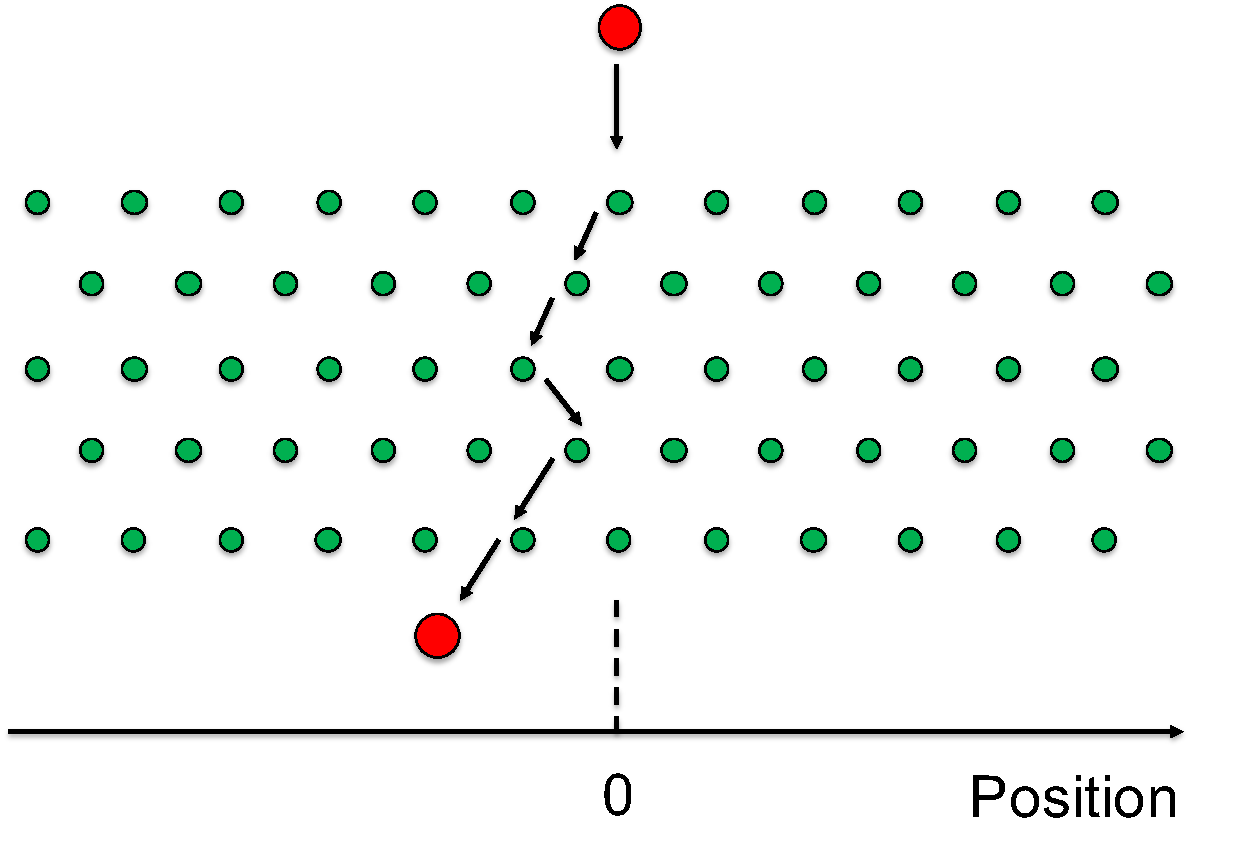
\includegraphics[width=0.6\textwidth]{figures/Probability/galton_image.pdf}
    \caption{The Galton machine: The idea is to drop the red counter down and let it work its way to the bottom. Each green pin will knock the counter left (-1 to its position) or right (+1 to its position) with an equal probability for each. At the end we'll count how many counters are at each position.}
    \label{fig:galton}
\end{figure}

\begin{figure}[hbt!]
    \centering
    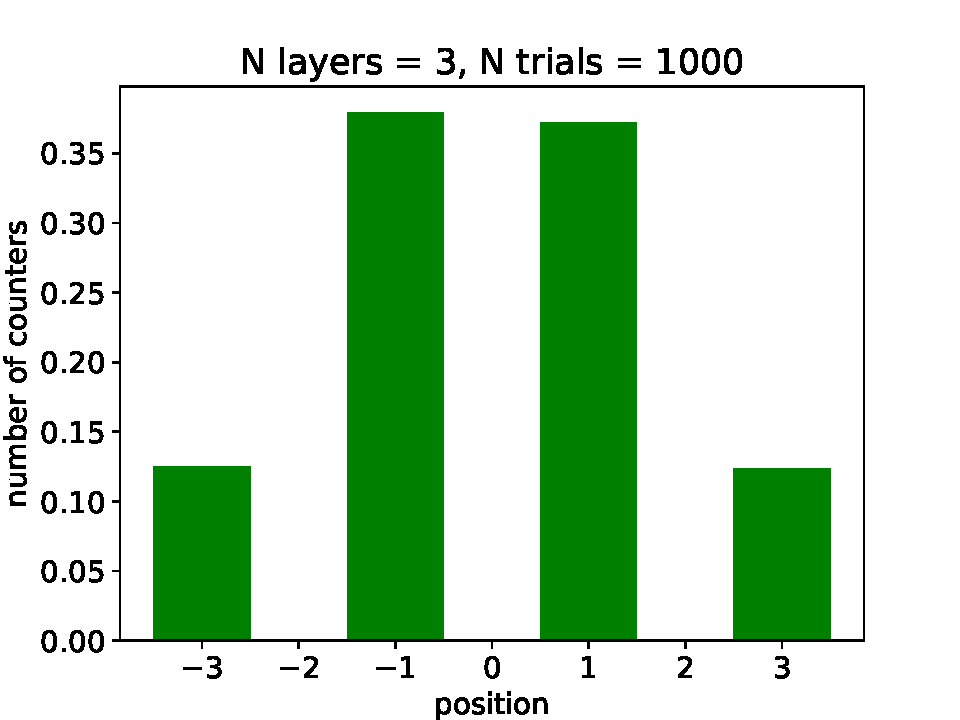
\includegraphics[width=0.32\textwidth]{figures/Probability/layers3.pdf}
    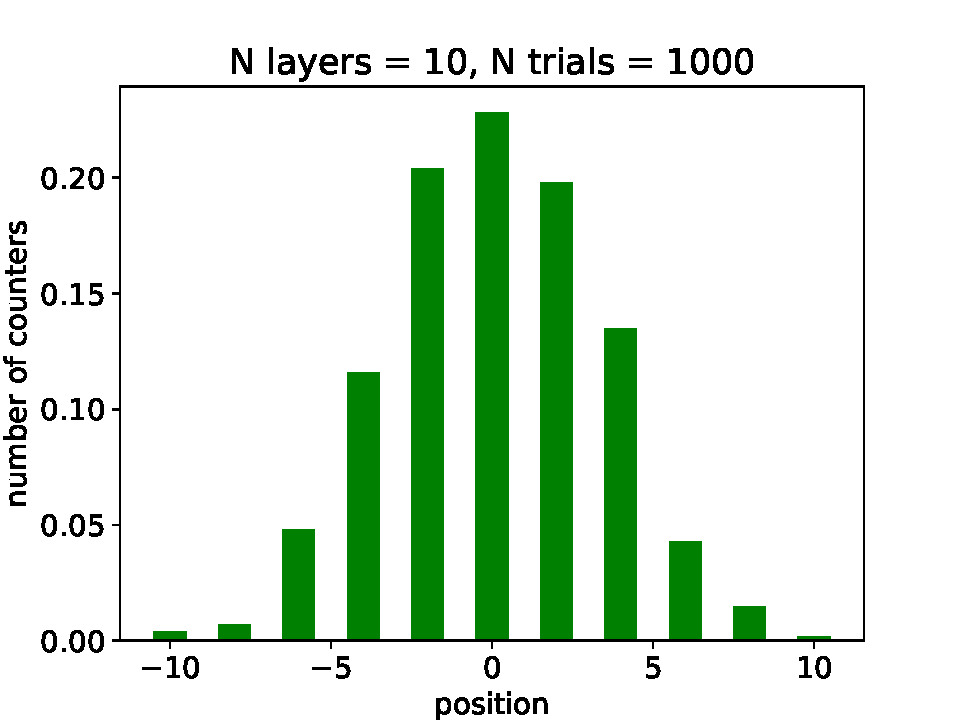
\includegraphics[width=0.32\textwidth]{figures/Probability/layers10.pdf}
    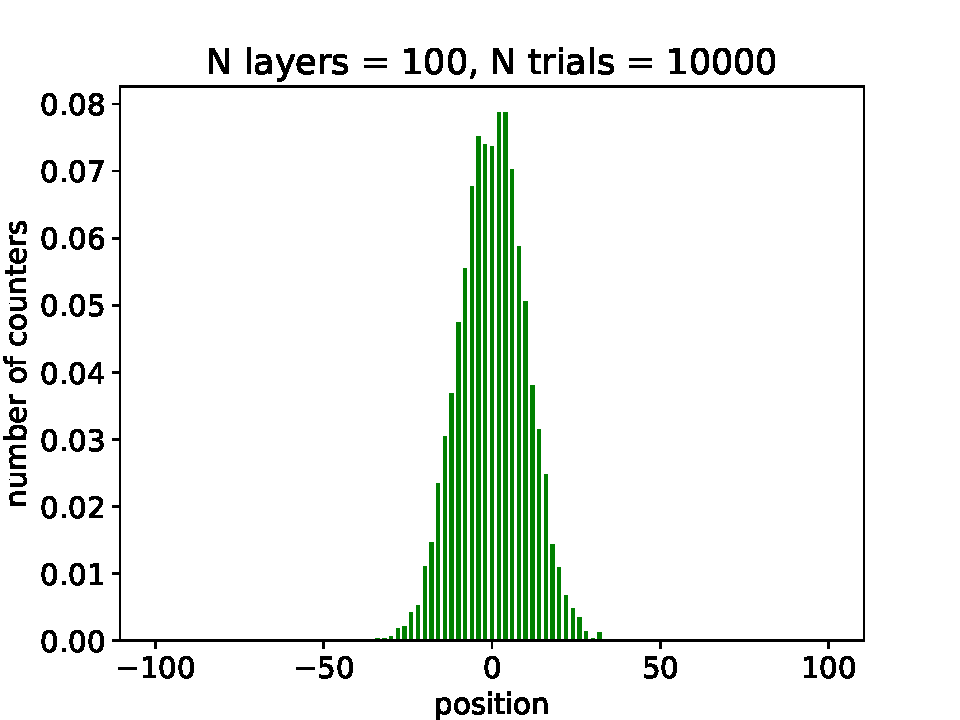
\includegraphics[width=0.32\textwidth]{figures/Probability/layers100.pdf}
    \caption{Galton machine simulation for 3, 10 and 100 layers. As the number of layers increases, we need more trials (counters) to fill in the possible positions but also we start to see the Gaussian distribution appear.}
    \label{fig:simgalton}
\end{figure}

\subsection{Markov Chains}

In the next section, we will discuss how distribtuions of random 
variables are used in quantifying the compatibility of what we observe 
in experiment with what we might expect to see given a theoretical 
model (for example the Standard Model) -- this is Hypothesis testing. 
Before we do, it is worth mentioning that analytic expressions for 
these distributions may not always be easy to calculate and certainly 
are often less computationally efficient than MC methods. 

We've already come across a MC process in the previous 
example of the Galton machine to build a Gaussian distribution. In this 
example, each MC sample (each counter dropped) is independent. For problems 
with low numbers of dimensions, these kinds of processes are 
capable of accurately determining the probability distribution. However, 
as the number of dimensions grows, we begin to encounter the so called 
\emph{``curse of dimensionality''}, where the number of independent 
samples needed to acccurately sample the space grows to the power of 
the number of dimensions!

We can be more efficient in how we sample to improve the situation. There 
are many ways to do this (enough to fill a whole lecure series), but 
as an example, we'll take a look at one commonly used in Bayesian statistics -- 
``Markov chains''. 

Broadly (and as Wikipedia defines it), A Markov chain 
is a stochastic model describing a sequence of possible events 
in which the probability of each event depends only on the state 
attained in the previous event. Practically for us this means we 
can use information about the previous MC sample to better choose 
the next one. This approach is very common in determining the  
posterior distribution from Bayes' theorem (see 
equation~\ref{eqn:bayesexp}). 

There are several algorithms that implement Markov chains 
but one which is used often in Bayesian statistics is the ``Metropolis-Hastings'' 
algorithm which works as follows; 

\begin{itemize}
 \item{
    We begin with an initial value for $\theta$. Ideally this should 
    be somewhere in a reasonable range for the parameter. 
 }
 \item{
     First we randomly pick values of $\theta$, 
    from a proposal generating function 
    $P(\theta_{\text{new}}|\theta_{\text{new}})$. This can be any 
    function that satisifes $P(A|B) = P(B|A)$. A common choice is to 
    use a Gaussian probability $\theta_{\text{new}}\sim \phi(\theta,1)$.
    }
\item{
    Next we need to decide whether to accept the proposed next value 
    for $\theta$ or stick to the original value and reject the new step. 
    For this we use the ratio of the posterior probability 
    between the current value of the parameter 
    ($\theta$) and the proposed one ($\theta_{\text{new}}$). 
    We define the ratio, 
    $r(\theta_{\text{new}},\theta) = \frac{p(\theta_{\text{new}}|X)}{p(\theta|X)} = \frac{p(X|\theta_{\text{new}})p(\theta_{\text{new}})}{p(X|\theta)p(\theta)}$
}
\item{
    The decision to accept or reject the value will be determined 
    by the value of $r$. If $r>1$ - accept $\theta_{new}$, otherwise,
}
  \begin{itemize}
  \item{else} 
     \item{define $\alpha = \text{min}(r,1)$}
     \item{draw a random uniform value between 0 and 1 , $t\sim U(0,1)$. }
     \item{if $t<\alpha$, accept $\theta_\text{new}$ as the 
     new value of $\theta$, otherwise reject it and 
     keep $\theta$ as the value.}
  \end{itemize} 
\item{With the new value accepted  or rejected, return  to the start  
with either the initial value now set to $\theta_\text{new}$ or 
the current one, depending on the outcome of the previous step.}
\end{itemize}

You can see that the accepted values of the parameter $\theta$ forms a 
chain of values and each step in this chain is a MC sample. Note that 
because of the way the chain is generated, these  samples are \emph{not} 
independent!

Of course, the best way to see this is with an example.   

\begin{tcolorbox}[colback=backblue]
    \textbf{Example:} Let's take a simple example 
    where $X\sim \phi(\theta,1)$ - is normally 
    distributed and $p(\theta)=phi(0.5,2)$. Suppose 
    our data is represented by a single measurement of $X=1.2$.

    Our prior is,
    
    \begin{equation}
    p(\theta)\propto e^{-\frac{1}{2}\frac{(\theta-0.5)^{2}}{2^{2}}}
    \end{equation}
    
    and the \emph{likelihood} is, 
    
    \begin{equation}
    p(X|\theta)\propto e^{-\frac{1}{2}\frac{(1.2-\theta)^{2}}{1^{2}}}
    \end{equation}
    
    where we've ignored the normalisation term since it will cancel 
    in the ratio. We can calculate the posterior analytically in this 
    case and check the outcome  of our Markov chain algorithm. 

    The notebook \href{https://github.com/nucleosynthesis/PGStatistics/blob/main/notebooks/MarkovChainMCExample.ipynb}{MarkovChainMCExample.ipynb} 
    will produce Figure~\ref{fig:mcmcmhex}. The histogram is generated 
    from the Markov chain process using the Metropolis-Hastings algorithm 
    while the red line is the direct calculation. 
\end{tcolorbox}

\begin{figure}[hbt!]
    \centering
    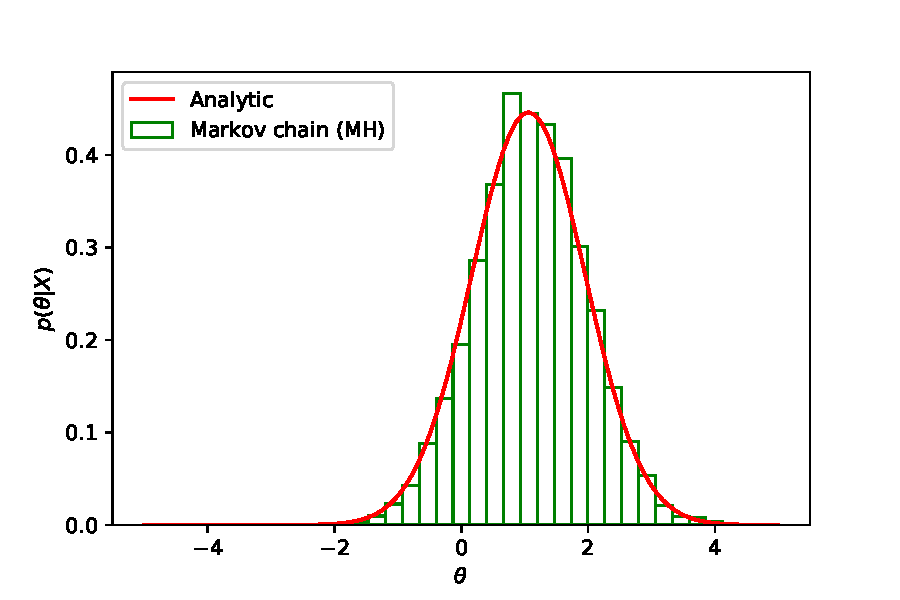
\includegraphics[width=\textwidth]{figures/Probability/markovchainexample.pdf}
    \caption{Posterior distribution  for simple Gaussian process. 
    The histogram is generated 
    from the Markov chain process using the 
    Metropolis-Hastings algorithm 
    while the red line is the direct calculation. }
    \label{fig:mcmcmhex}
\end{figure}
